\chapter{Results}
\label{chap:res}

\begin{markdown}

The following sections describes results when comparing the proposed
PTX.jl library to the existing alternatives for Julia. The
alternatives explored are the CUDA and OpenCL bindings, provided as
external Julia modules through the package management system. The
kernels used marked with OpenCL and CUDA are written in C. In
addition, a comparison to the Julia core math library is presented.
Section \ref{sec:res:productivity} includes a small analysis of
programmer productivity.

# Benchmarks #
\label{sec:res:bench}

\begin{table}[H]
  \centering
  \begin{tabular}{|l|l|}
    \hline
    Application & Name \\
    \hline
    Image Processing & Gaussian Blur \\
    \hline
    Linear Algebra & General Matrix Multiplication \\
    \hline
  \end{tabular}
  \caption{Benchmarks}
  \label{res:benchmarks}
\end{table}

The benchmarks presented in Table \ref{res:benchmarks} are well known
and general compute kernels. Both benchmarks are implemented naively,
meaning no special optimization are applied. This is done to make the
implementation easily comparable. Note that the CPU implementation of
the Matrix Multiplication benchmark is part of the optimized Julia
core math library, and this should be taken into consideration when
comparing CPU and GPU performance.

# Method and Measurement #
\label{sec:res:measure}

The benchmarks are executed with the same randomly generated input
data. For each problem size, the kernel is executed 100 times and the
average running time is reported.

# Gaussian Blur #

The Gaussian blur kernel is a common image processing operation. With
this benchmark, we compare the performance of the Julia kernel compared
to kernel implementations in CUDA C and OpenCL C. All three kernels are
scheduled using the Julia CUDA or OpenCL bindings. 

## Evaluation of correctness ##

To evaluate the correctness of the benchmark a test set of 256*256
floating point numbers were generated and the kernel was executed once
for each implementation. Table \ref{tab:res:blur:diff} show the the
sum of the element-wise difference for the PTX.jl implementation
compared to OpenCL and CUDA.

\begin{table}[H]
  \centering
  \begin{tabular}{|l|r|r|}
    \hline
    Data type & OpenCL vs PTX.jl & CUDA vs PTX.jl \\
    \hline
    Float32  & 0.0 & 0.0 \\
    \hline
  \end{tabular}
  \caption{Element-wise difference of a 256*256 blur filter compared to PTX.jl}
  \label{tab:res:blur:diff}
\end{table}

Table \ref{tab:res:blur:diff} shows that all the three implementations
are functionally equivalent.

## Visual evaluation of correctness ##

As the previous evaluation of correctness could include the same error
propagated through all the implementation we consider a visual
evaluation as well. The visualization is easier to verify. The kernels
are executed on an input image and the result is shown in Figure
\ref{fig:res:blur:pic}.

\begin{figure}[H]
  \centering
  \begin{subfigure}{.49\textwidth}
    \centering
    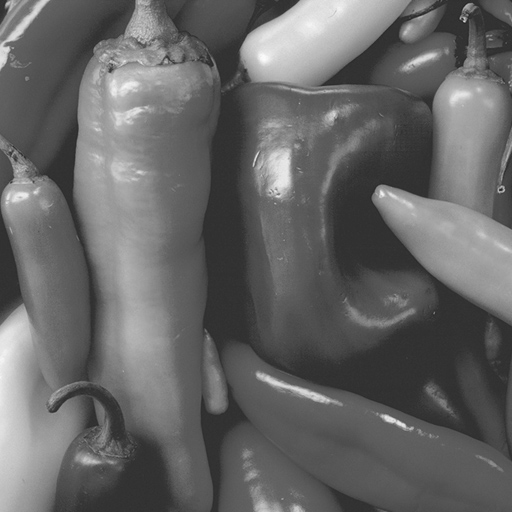
\includegraphics[width=1\textwidth]{body/figures/results/blur/input.png}
    \caption{Original image}
    \label{fig:res:blur:pic:input}
  \end{subfigure}%
  \hspace{.01\textwidth}
  \begin{subfigure}{.49\textwidth}
    \centering
    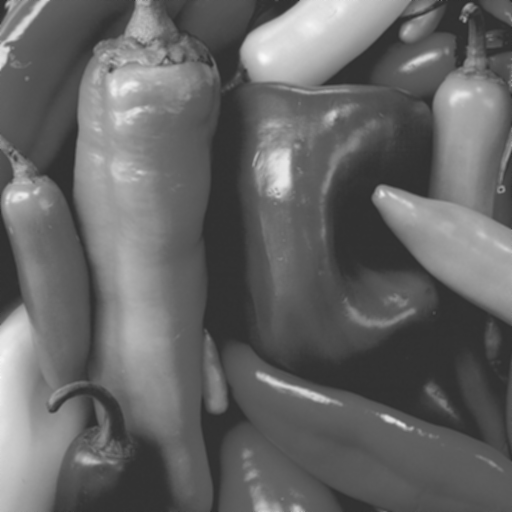
\includegraphics[width=1\textwidth]{body/figures/results/blur/cuda.png}
    \caption{CUDA}
    \label{fig:res:blur:pic:cuda}
  \end{subfigure}%
  \hspace{.01\textwidth}
  \begin{subfigure}{.49\textwidth}
    \centering
    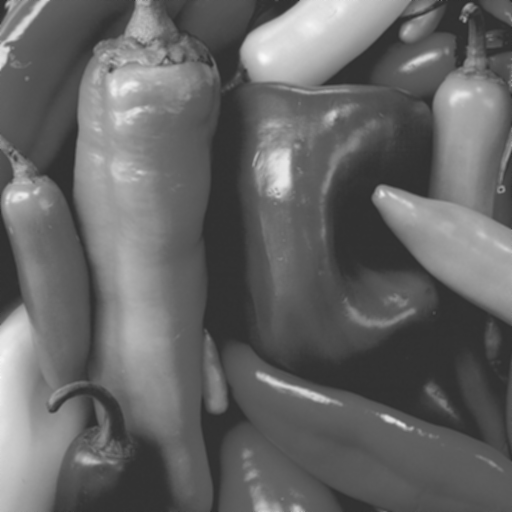
\includegraphics[width=1\textwidth]{body/figures/results/blur/julia.png}
    \caption{PTX.jl}
    \label{fig:res:blur:pic:julia}
  \end{subfigure}%
  \hspace{.01\textwidth}
  \begin{subfigure}{.49\textwidth}
    \centering
    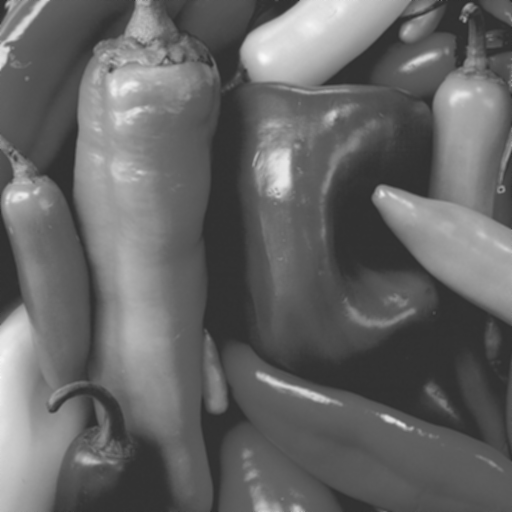
\includegraphics[width=1\textwidth]{body/figures/results/blur/opencl.png}
    \caption{OpenCL}
    \label{fig:res:blur:pic:opencl}
  \end{subfigure}
  \caption{Blur filter applied to a gray-scale image}
  \label{fig:res:blur:pic}
\end{figure}

By examining the pictures in Figure \ref{fig:res:blur:pic}, we can see
that each implementation has the same and correct blur effect on the
original image in \ref{fig:res:blur:pic:input}.

## Performance evaluation ##
\label{sec:res:blur:perf}

The performance is recorded as described in Section
\ref{sec:res:measure}. The result is presented in Figure \ref{fig:res:blur}.

\begin{figure}[H]
  \centering
  \begin{subfigure}{.33\textwidth}
    \centering
    \includegraphics[width=1\textwidth]{body/results/blur/mem.png}
    \caption{Memory Transfer}
    \label{fig:res:blur:int32:mem}
  \end{subfigure}%
  \begin{subfigure}{.33\textwidth}
    \centering
    \includegraphics[width=1\textwidth]{body/results/blur/exec.png}
    \caption{Execution time}
    \label{fig:res:blur:int32:exec}
  \end{subfigure}%
  \begin{subfigure}{.33\textwidth}
    \centering
    \includegraphics[width=1\textwidth]{body/results/blur/total.png}
    \caption{Total Time}
    \label{fig:res:blur:int32:tot}
  \end{subfigure}%
  \caption{Performance of Blur kernel}
  \label{fig:res:blur}
\end{figure}

Figure \ref{fig:res:blur} reveals the fact that the kernels generated
by PTX.jl is comparable to CUDA and OpenCL. Comparing the execution
time of CUDA and PTX.jl, we see that they are equal for all input
sizes. The OpenCL kernel performes slightly worse than the other
kernels. The jump in Memory Transfer time at approximately n = 2500
seems to be related to the implementation between the CPU and GPU. The
jump is observed for the same input size for both benchmarks and both
the CUDA and OpenCL bindings.

# Matrix Multiply #
\label{sec:res:mm}

The Matrix Multiplication benchmark is a simple $C = A * B$ matrix
multiplications, where $A, B, C$ all are $n*n$ matrices. The benchmark
is executed for all the supported data types, 32 and 64 bits integer
and floating point numbers. We here compare the Julia kernel to a CPU
implementation and a CUDA kernel created by the __nvcc__ compiler.
The CPU implementation is simply the matrix multiply operator in the
Julia language. Therefore the memory overhead for the CPU version is
zero. We look at the differences between floating point and integer
performance.

## Integer ##

Figures \ref{fig:res:mm:int32} and \ref{fig:res:mm:int64} shows the
average execution time when the problem size is varied. The section is
chosen to describe the point where computing the product goes from
being faster on the CPU to being faster on the GPU.

\begin{figure}[H]
  \centering
  \begin{subfigure}{.33\textwidth}
    \centering
    \includegraphics[width=1\textwidth]{body/results/mm/int32-mem.png}
    \caption{Memory Transfer}
    \label{fig:res:mm:int32:mem}
  \end{subfigure}%
  \begin{subfigure}{.33\textwidth}
    \centering
    \includegraphics[width=1\textwidth]{body/results/mm/int32-exec.png}
    \caption{Execution Time}
    \label{fig:res:mm:int32:exec}
  \end{subfigure}%
  \begin{subfigure}{.33\textwidth}
    \centering
    \includegraphics[width=1\textwidth]{body/results/mm/int32-total.png}
    \caption{Total Time}
    \label{fig:res:mm:int32:tot}
  \end{subfigure}
  \caption{32-bit Integer}
  \label{fig:res:mm:int32}
\end{figure}

\begin{figure}[H]
  \centering
  \begin{subfigure}{.33\textwidth}
    \centering
    \includegraphics[width=1\textwidth]{body/results/mm/int64-mem.png}
    \caption{Memory Transfer}
    \label{fig:res:mm:int64:mem}
  \end{subfigure}%
  \begin{subfigure}{.33\textwidth}
    \centering
    \includegraphics[width=1\textwidth]{body/results/mm/int64-exec.png}
    \caption{Execution Time}
    \label{fig:res:mm:int64:exec}
  \end{subfigure}%
  \begin{subfigure}{.33\textwidth}
    \centering
    \includegraphics[width=1\textwidth]{body/results/mm/int64-total.png}
    \caption{Total Time}
    \label{fig:res:mm:int64:tot}
  \end{subfigure}
  \caption{64-bit Integer}
  \label{fig:res:mm:int64}
\end{figure}

The _Memory Transfer_ in Figure \ref{fig:res:mm:int32:mem} and
\ref{fig:res:mm:int64:mem} reveals no surprises. The CPU does not
require any memory transfer, therefore the graph is not visible in the
figures. As expected, both CUDA and PTX.jl exposes a steady increase
as the problem size grows.

We see a radical difference in the scaling properties of the CPU
versus GPU implementation in Figures \ref{fig:res:mm:int32:exec} and
\ref{fig:res:mm:int64:exec}. This is expected, considering the number
of cores on the GPU is two orders of magnitude lager than the CPU. We
see that by only considering execution time, the GPU implementation
surpass the CPU at $n=50$ for 32-bits, and at $n=38$ for 64-bits.

## Floating point ##

\begin{figure}[H]
  \centering
  \begin{subfigure}{.33\textwidth}
    \centering
    \includegraphics[width=1\textwidth]{body/results/mm/float32-mem.png}
    \caption{Memory Transfer}
    \label{fig:res:mm:float32:mem}
  \end{subfigure}%
  \begin{subfigure}{.33\textwidth}
    \centering
    \includegraphics[width=1\textwidth]{body/results/mm/float32-exec.png}
    \caption{Execution Time}
    \label{fig:res:mm:float32:exec}
  \end{subfigure}%
  \begin{subfigure}{.33\textwidth}
    \centering
    \includegraphics[width=1\textwidth]{body/results/mm/float32-total.png}
    \caption{Total Time}
    \label{fig:res:mm:float32:tot}
  \end{subfigure}
  \caption{32-bit Floating point}
  \label{fig:res:mm:float32}
\end{figure}


\begin{figure}[H]
  \centering
  \begin{subfigure}{.33\textwidth}
    \centering
    \includegraphics[width=1\textwidth]{body/results/mm/float64-mem.png}
    \caption{Memory Transfer}
    \label{fig:res:mm:float64:mem}
  \end{subfigure}%
  \begin{subfigure}{.33\textwidth}
    \centering
    \includegraphics[width=1\textwidth]{body/results/mm/float64-exec.png}
    \caption{Execution Time}
    \label{fig:res:mm:float64:exec}
  \end{subfigure}%
  \begin{subfigure}{.33\textwidth}
    \centering
    \includegraphics[width=1\textwidth]{body/results/mm/float64-total.png}
    \caption{Total Time}
    \label{fig:res:mm:float64:tot}
  \end{subfigure}
  \caption{64-bit Floating point}
  \label{fig:res:mm:float64}
\end{figure}

For the floating point benchmarks we see a different picture compared
to their integer counterparts. The computations actually scales
equally well on the CPU as on the GPU. With the CPU having a 1.3x
advantage for $n=4096$ on single precision and the GPU at 1.4X on
double precision.

The significant increase in memory access time is commented in
Section \ref{sec:res:blur:perf}.

# Programmer Productivity #
\label{sec:res:productivity}

The \gls{LOC} metric is a widely used measurement of the complexity of
a computer program. Minimizing this metric can lead to increased
programmer productivity.

## LOC ##
\label{sec:res:loc}

Table \ref{tab:loc} tabulates the LOC for the kernels for the two
benchmarks presented in Chapter \ref{sec:res:bench}.

\begin{table}[H]
  \centering
  \begin{tabular}{|l|l|l|l|l|}
    \hline
    & \textbf{CPU} & \textbf{OpenCL C} & \textbf{CUDA C} & \textbf{PTX.jl} \\
    \hline
    Gaussian Blur   & N/A & 19       & 19     & 19 \\
    \hline
    Matrix Multiply & 588 & N/A      & 19     & 22 \\
    \hline
  \end{tabular}
  \caption{Lines of Code in kernels}
  \label{tab:loc}
\end{table}

The results in Table \ref{tab:loc} shows that the LOC was not reduced
for any of the kernels compared to OpenCL and CUDA C. For the CPU
implementation, the count is the entire _base/linalg/matmul.jl_
implementation. This is included to indicate the size of an optimized
implementation. The implementations for OpenCL, CUDA and PTX.jl are
not optimized.

## Dynamic Typing ##

The fact that the kernels implemented with PTX.jl are written in a
dynamic language, enables one kernel definition to handle multiple
primitive types. This causes the Matrix Multiplication benchmark to be
implemented as one kernel, while the CUDA C has to be implemented
with one kernel per type, totaling in four implementations.

\end{markdown}
